\documentclass{beamer}
% xelatex 
\usepackage[ngerman]{babel}
\usepackage[backend=biber]{biblatex}
\usepackage{fontspec}
\usepackage{graphicx}
\usepackage{csquotes}
\usepackage{lmodern}
\usepackage{tikz}
\usetikzlibrary{shapes.geometric, arrows.meta}


%\setmainfont{Fira Sans}
\setmonofont{Fira Code}
%\setsansfont{Fira Sans}
\author{Jasper Levin Spahl}

\title{Der Smarte Bienenstock}
\subtitle{Entwicklung eines Serversystems}

\logo{
\includegraphics[width=1.575cm]{qrcode.png}}

\usetheme{Berlin}
\usecolortheme{beaver}

\begin{document}

\begin{frame}
	\titlepage{}
\end{frame}


\section*{Überblick}

\begin{frame}{Überblick}
	\only<1>{Warum ist da ein QR Code?}
	\only<2>{\tableofcontents}
\end{frame}

\section{Einleitung}

\begin{frame}
	\frametitle{Einleitung}	
	\begin{itemize}
		\item<1-> Wie kam ich auf das Thema?
		\item<2-> ``Das gibt's doch schon, warum mach ich mir dann den Aufwand?''
		
	\end{itemize}
\end{frame}

\section{Open Source}

\subsection{Was ist Open Source?}

\begin{frame}
	
\includegraphics[width=\textwidth]{opensource.png}
\end{frame}

\subsection{Warum ist das wichtig?}

\begin{frame}{Warum ist das wichtig?}
	\begin{itemize}
		\item<2-> man kann sehen was im Hintergrund passiert
		\item<3-> Corona App
		\item<4-> wenn dir was nicht passt kannst du es ändern
		\item<5-> das Ziel ist nicht Geld zu verdienen
	\end{itemize}
\end{frame}

\section{Konzepte und Begriffe}
	
\begin{frame}{Was ist ein Server?}
	\begin{block}{Frage}
		Auf welchem der folgenden Bildern ist kein Server zu sehen.
	\end{block}
	\only<2->{
	\begin{columns}
		\column{.5\textwidth}
		\centering
		\includegraphics[height=.3\textheight]{Wikimedia_Foundation_Servers-8055_35.jpg}
		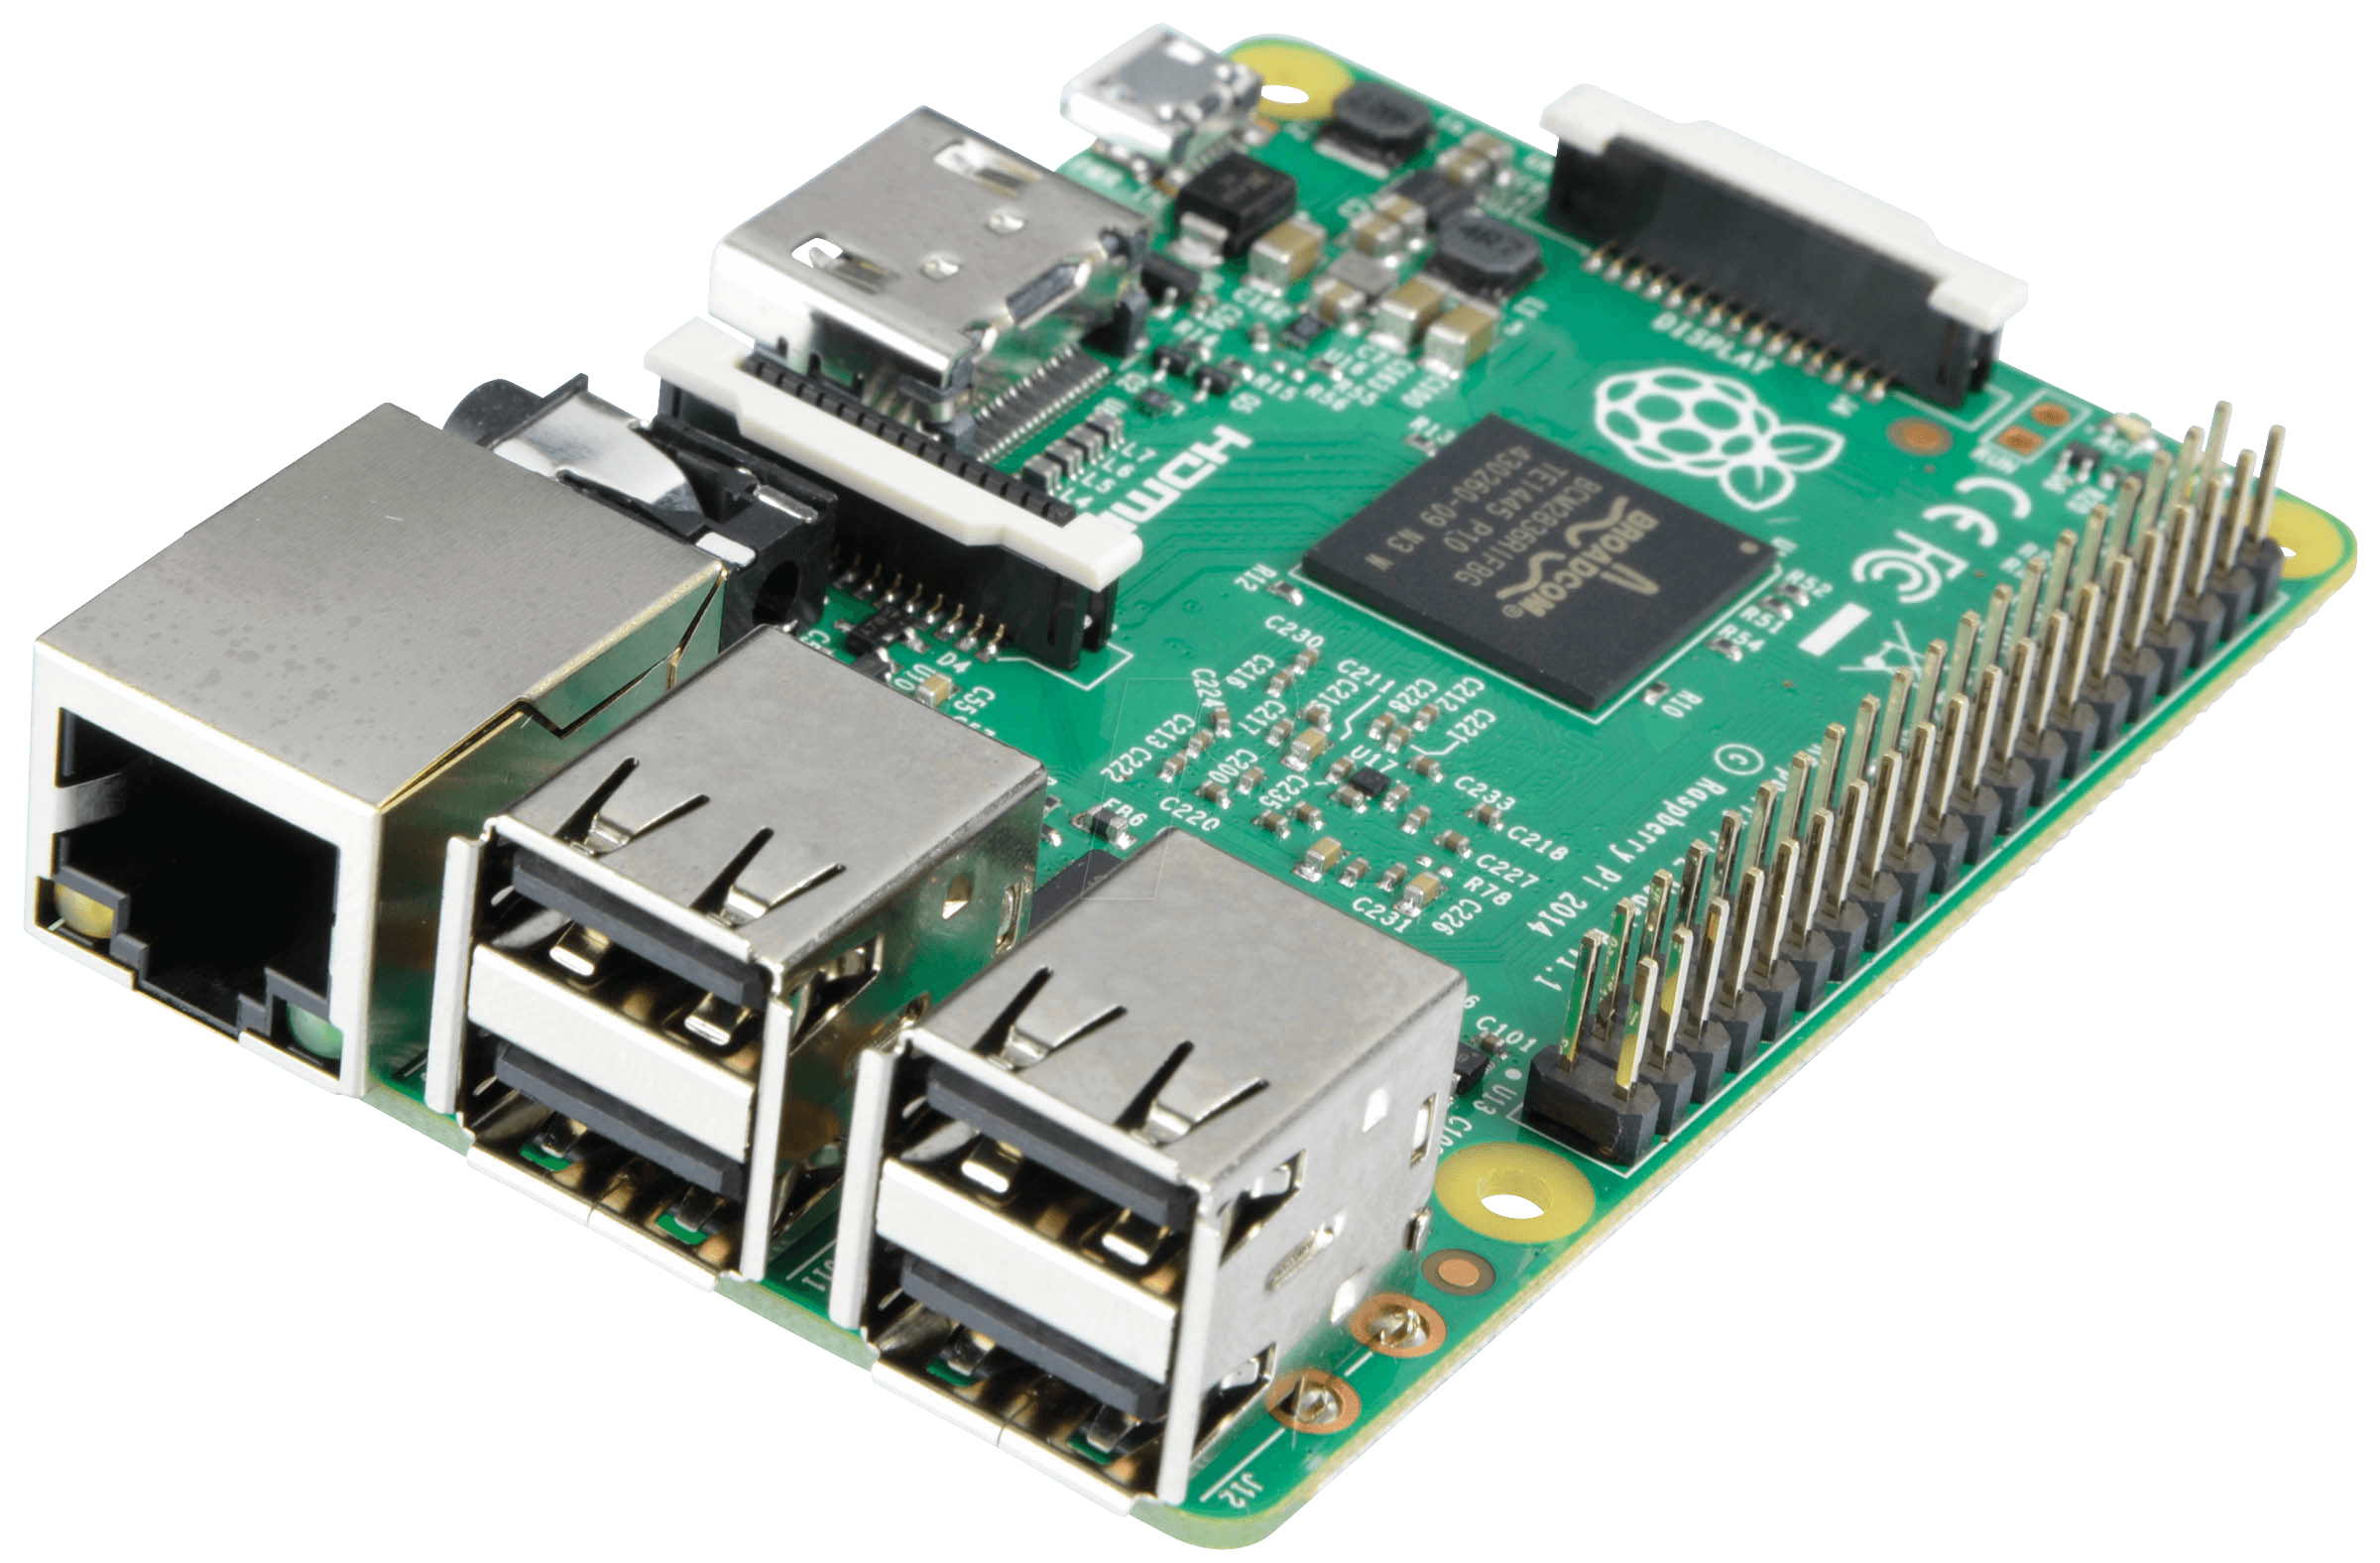
\includegraphics[height=.3\textheight]{rapi.png}
		\column{.5\textwidth}
		\centering
		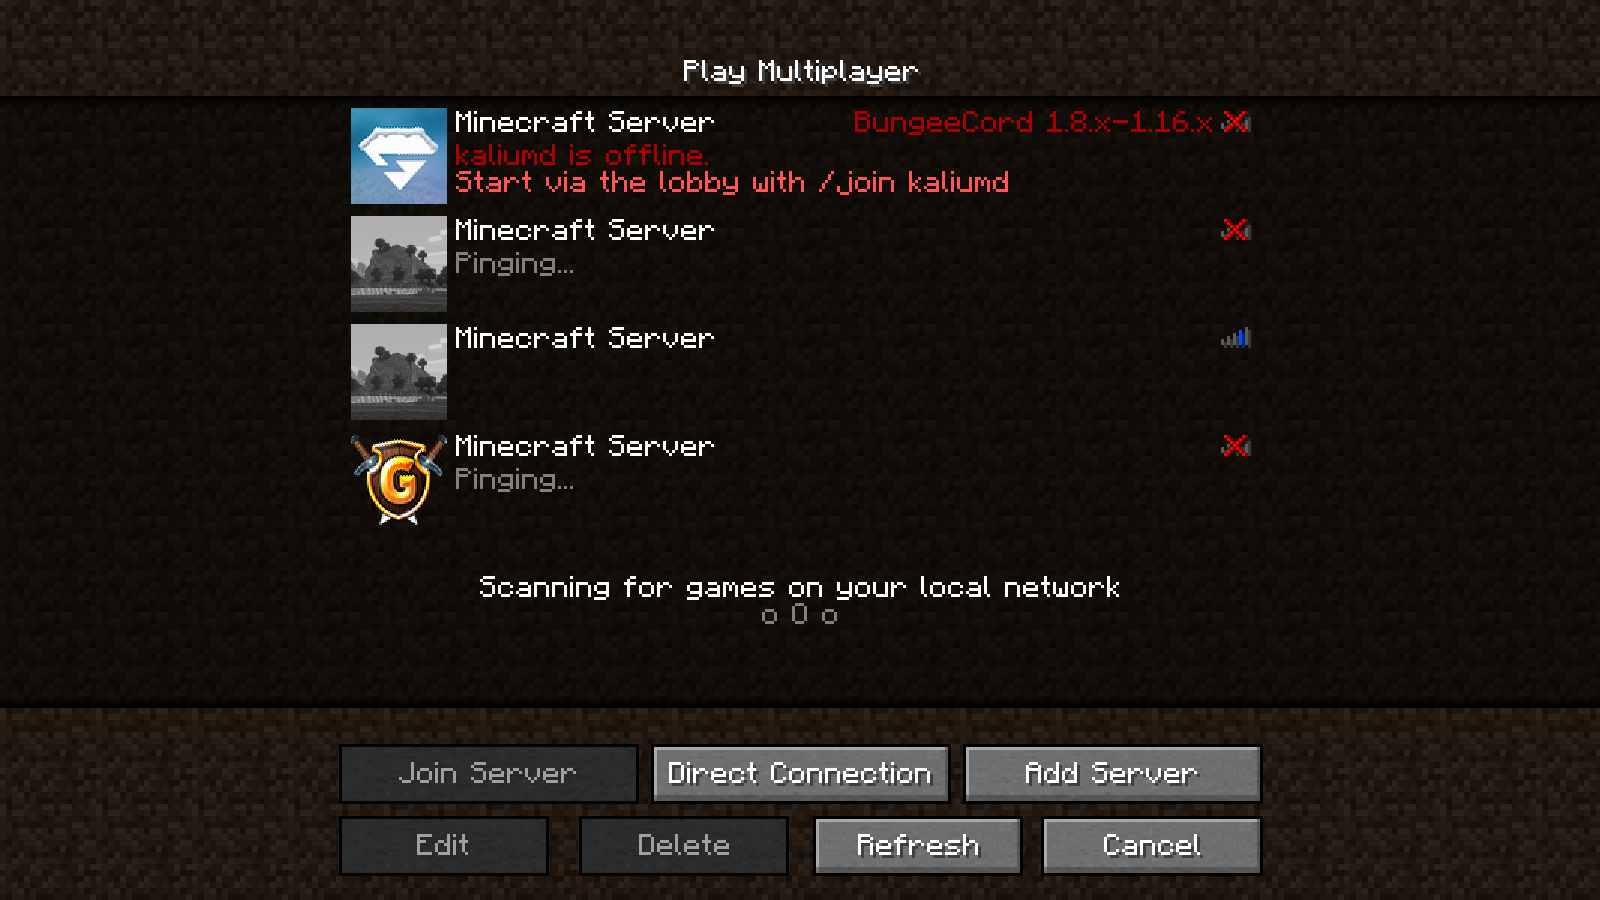
\includegraphics[height=.3\textheight]{Serverlist.png}
		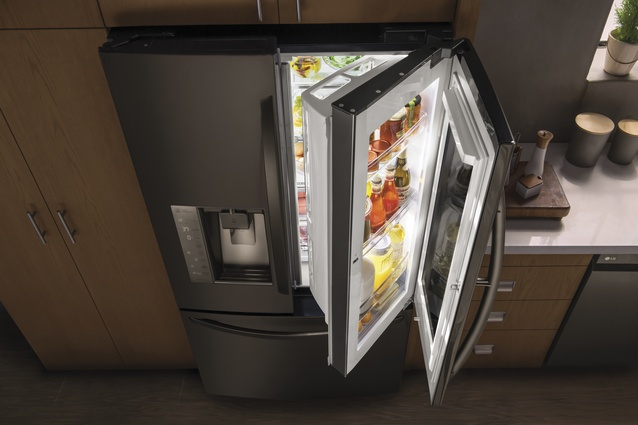
\includegraphics[height=.3\textheight]{qwe_download.jpg}
	\end{columns}
	}
\end{frame}

\begin{frame}{Was ist ein Server?}
	\begin{alertblock}{Wichtig}
		Es gibt zwei verschiedene Arten von Servern!
	\end{alertblock}

	\begin{itemize}
		\item<2-> Der Hardwareserver
			\only<3-5>{\begin{itemize}
				\item<3-> Host
				\item<4-> Ein Gerät, auf dem ein Serversoftware läuft
				\item<5>[$\Downarrow$]
				\item<5> Fast alles kann ein Server sein
			\end{itemize}}
	\item<6-> Der Softwareserver
		\begin{itemize}
			\item<7-> Ein Programm
			\item<8-> Stellt Dienste zur Verfügung
			\item<9-> z.B. Eine Webseite
			
		\end{itemize}
	\end{itemize}
\end{frame}

\begin{frame}{Was ist eine API?}
	\begin{itemize}
		\item<2-> \emph{Application Programming Interface}
		\item<3-> \emph{Anwendungsprogrammierschnittstelle}
		\item<4-> Ermögliche Kommunikation zwischen Programmen
		\item<5-> Unterschiedlich je nach Anwendung
	\end{itemize}
\end{frame}

\section{Die Bienenstockwaage}
\begin{frame}{Die Bienenstockwaage}
	\begin{block}{Frage}
		Was ist eine Bienenstockwaage?
	\end{block}
	\begin{exampleblock}<2->{Antwort}
		Waage unter einem Bienenstock
	\end{exampleblock}
\end{frame}

\begin{frame}{Funktionsweise}
	\centering	
	\begin{tikzpicture}
		\node[draw] (waage1) at (0,0) {Waage 1};
		\node[draw] (waage2) [below of = waage1] {Waage 2};
		\node[draw=none] (waage3) [below of = waage2, below = -0.5cm] {...};
		\node[draw] (waagen) [below of = waage3, below = -0.6cm] {Waage $n$};
		\node[draw, shape=circle] (server) [right of = waage2, right = 2cm] {Webserver};
		\node[draw] (app)    [below of = server, below = 0.7cm] {Webseite};
		\node[draw] (data)   [right of = server, right = 1.5cm] {Datenbank};

		\draw[-Stealth] (waage1) -- (server);
		\draw[-Stealth] (waage2) -- (server);
		\draw[-Stealth] (waagen) -- (server);
		\draw[Stealth-Stealth] (server) -- (data);
		\draw[Stealth-Stealth] (app) -- (server);
	\end{tikzpicture}

\end{frame}

\section{Demonstration}
\section{Fragen}
	
\begin{frame}
	\Huge{Habt Ihr Noch Fragen?}
\end{frame}

\end{document}
